% !TEX program = xelatex -> bibtex -> xelatex*2

\documentclass[12pt]{ctexart}  
% ctexart支持中文编译文档
%最后全部翻译成英文后可以选择改成article,然后用pdflatex编译,还可以检验一下是不是没有中文了嘿嘿( •̀ ω •́ )✧
%官方要求字号不小于 12 号,此处选择 12 号字体

\CTEXsetup[format={\Large\bfseries}]{section} %在ctexart中,一级标题是居中的,这里改成左对齐

%% 本模板不需要填写年份,以当前电脑时间自动生成

%% 请在以下的方括号中填写队伍控制号
\usepackage[2401234]{ldmcm}  % 载入ldmcm模板文件
\problem{A}  % 请在此处填写题号

%%字体选择
%\usepackage{mathptmx}  % 这是 Times 字体,中规中矩 
\usepackage{mathpazo}  % 这是 COMAP 官方杂志采用的更好看的 Palatino 字体,可替代以上的 mathptmx 宏包

%%几处小修改,如无特殊需求可不做更改
\newcommand{\upcite}[1]{\textsuperscript{\textsuperscript{\cite{#1}}}}%这是参考文献引用上标的命令
\graphicspath{{img/}}          % 此处{img/}为相对路径,注意加上“/”
\let\itemize\compactitem
\let\enditemize\endcompactitem%解决列表环境中行距过大的问题

\title{Here is Your Title}  % 标题

% 如需要修改题头(默认为 MCM /ICM),请使用以下命令(此处修改为 MCM)
%\renewcommand{\contest}{MCM}

% ----------------------------------------------文档开始---------------------------------------------------------
\begin{document}

% 此处填写摘要内容-----------摘要摘要摘要摘要摘要摘要摘要摘要摘要摘要摘要摘要摘要摘要摘要摘要摘要摘要摘要摘要摘要
\begin{abstract}
	%第一段:2句话背景+2句话概括全文完成的任务
	Global warming, El Niño... With the emergence of various extreme climates,\textbf{Austral-ia's wildfires} occur more frequently. The greenhouse gases emitted after combustion have exacerbated global warming, which seems to have entered an endless loop. At the same time, hundreds of millions of lives have been killed in the fire, which makes us sad. To better control wildfires, we modeled the \textbf{distribution of drones} assisting in the observation to achieve the best balance between economy and efficiency.

	%第二段:总结我们用了什么模型
	Several models are established: Model I: Rasterized Multi-Objective Optimization Model; Model II: Model Verification Simulated by Poisson Process; Model III: Hovering Model Based on Tabu Search, etc.

	%接下来分别介绍模型与结果
	For Model I:
	Firstly,%首先,我们从哪里收集到了什么样的数据
	We find data。。。
	Then,%然后,基于什么样的原因,我们建立了什么模型
	we establish \textbf{model}。。。
	Next,%我们选择或者设计了什么算法
	we use Algorithm。。。
	Finally,%我们得到了什么样的结果
	%数值直接写出来,大量数据(表)或图片则说请参见(are shown in ...)图几
	%注意要用文字,不要使用符号
	it can be seen that。。。

	For Model II:
	Firstly,%首先,我们从哪里收集到了什么样的数据
	We find data。。。
	Then,%然后,基于什么样的原因,我们建立了什么模型
	we establish model。。。
	Next,%我们选择或者设计了什么算法
	we use Algorithm。。。
	Finally,%我们得到了什么样的结果
	%数值直接写出来,大量数据(表)或图片则说请参见(are shown in ...)图几
	%注意要用文字,不要使用符号
	it can be seen that。。。

	For Model III:
	Firstly,%首先,我们从哪里收集到了什么样的数据
	We find data。。。
	Then,%然后,基于什么样的原因,我们建立了什么模型
	we establish model。。。
	Next,%我们选择或者设计了什么算法
	we use Algorithm。。。
	Finally,%我们得到了什么样的结果
	%数值直接写出来,大量数据(表)或图片则说请参见(are shown in ...)图几
	%注意要用文字,不要使用符号
	it can be seen that。。。

	%灵敏度与稳健性分析
	Finally, sensitivity analysis 。。。 Meanwhile, robustness

	% 美赛论文中无需注明关键词。若一定要使用,
	% 请将以下两行的注释号 '%' 去除,以使其生效
	%\vspace{5pt}
	%\textbf{Keywords}: MATLAB, mathematics, LaTeX.

\end{abstract}

\maketitle  % 生成 Summary Sheet------------------------------------

\tableofcontents  % 生成目录


% -----------------------------------------正文开始-----------------------------------------------------------------------------------------------------------------------------------


%==============第一部分===引入=============================================================
\section{Introduction}
\subsection{Problem Background}%问题背景问题背景问题背景问题背景问题背景问题背景---------------------------------
一些常用的写作缩略语:

i.e.,。。。也即是。。。(一定加逗号)

e.g.,。。。例如,。。。

, etc.    。。。,等等。

n.b.   特别注意

cf.  参见


美赛一定要多上图,清晰直观,并且格式上最好是矢量图,例如pdf,而不是位图,例如jpg,png等,在形式上最好是组图,下面列出了利用\verb|subfigure|实现的
\verb|1x2,1x3,2x2|的几种组图:

%% 这是一个1x2的组图
\begin{figure}[htbp]
	\centering
	\begin{subfigure}[b]{.3\textwidth} %设置缩放比例,这里的.5代表缩放为原来的50%
		
\includegraphics[width=\textwidth]{img/example-image-a.pdf}
		\caption{left}\label{subfig:left}
	\end{subfigure}
	\hspace{10mm} %%%%%%%%%%%%%%%%%%调整子图间距
	\begin{subfigure}[b]{.3\textwidth}
		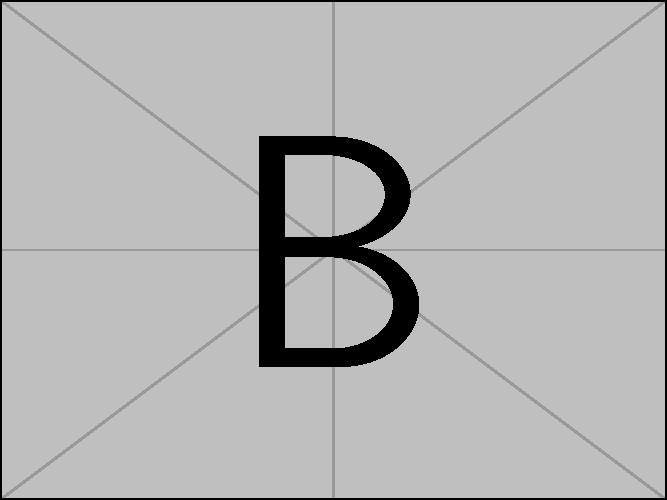
\includegraphics[width=\textwidth]{img/example-image-b.pdf}
		\caption{right}\label{subfig:right}
	\end{subfigure}
	\caption{Two images}\label{subfigure}
\end{figure}

Figure \ref{subfigure} gives an example of subfigures. Figure \ref{subfig:left} is on the left, and Figure \ref{subfig:right} is on the right.


%% 这是一个1x3的组图
\begin{figure}[!htbp]
	\centering
	\begin{subfigure}[t]{0.3\textwidth}
		\centering
		
\includegraphics[width=\textwidth]{img/example-image-a.pdf}
		\caption*{}
		\label{}
	\end{subfigure}
	\begin{subfigure}[t]{0.3\textwidth}
		\centering
		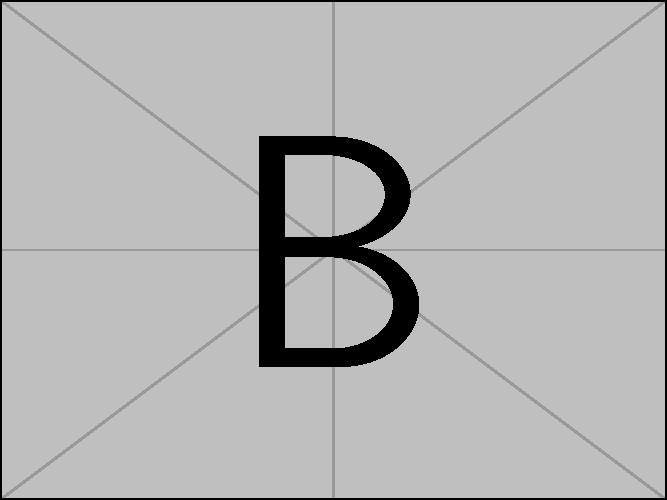
\includegraphics[width=\textwidth]{img/example-image-b.pdf}
		\caption*{}
		\label{}
	\end{subfigure}
	\begin{subfigure}[t]{0.3\textwidth}
		\centering
		
\includegraphics[width=\textwidth]{img/example-image-c.pdf}
		\caption*{}
		\label{}
	\end{subfigure}
	\caption{Three images}
	\label{Three images}
\end{figure}


%% 这是一个2x2的组图(可推广至2x3,3x3等)
\begin{figure}[!htbp]
	\centering
	\begin{subfigure}[t]{0.4\textwidth}
		\centering
		
\includegraphics[width=\textwidth]{img/example-image-a.pdf}
		\caption{左上}
		\label{}
	\end{subfigure}
	\begin{subfigure}[t]{0.4\textwidth}
		\centering
		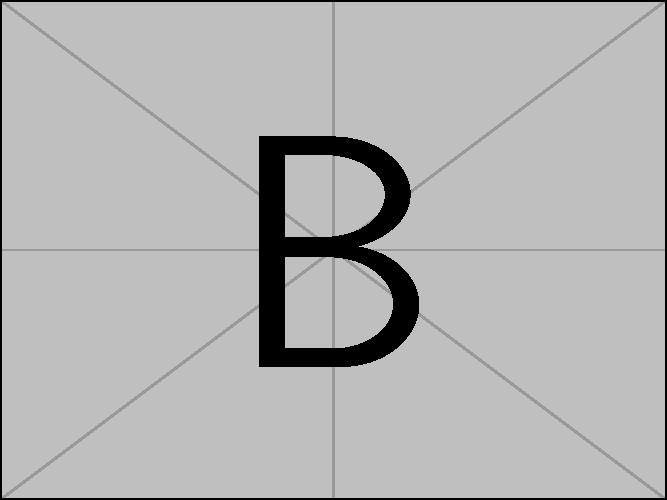
\includegraphics[width=\textwidth]{img/example-image-b.pdf}
		\caption{右上}
		\label{}
	\end{subfigure}
	%  \begin{subfigure}[t]{0.3\textwidth}
	%          \centering
	%          
\includegraphics[width=\textwidth]{img/example-image-a.pdf.pdf}
	%          \caption{}
	%          \label{}
	%  \end{subfigure}
	\qquad
	%%让图片换行,这就是实现多行组图的简单原理
	%%若需要搞一个2x3的组图就把上下的注释打开再添加图片就可以了
	%%注意调整比例以及间距
	\begin{subfigure}[t]{0.4\textwidth}
		\centering
		
\includegraphics[width=\textwidth]{img/example-image-a.pdf}
		\caption{左下}
		\label{}
	\end{subfigure}
	\begin{subfigure}[t]{0.4\textwidth}
		\centering
		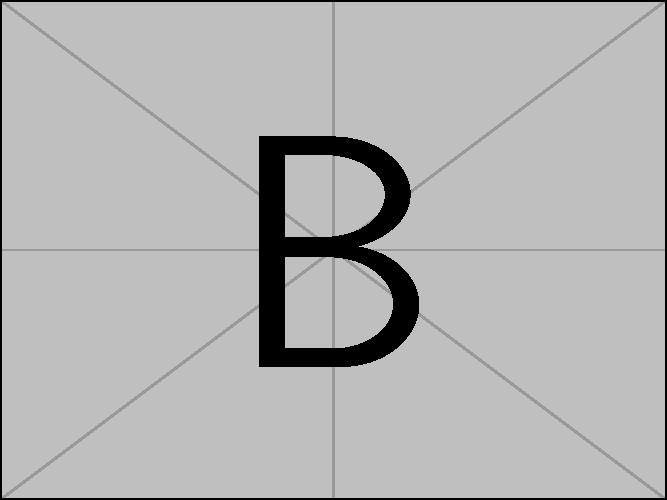
\includegraphics[width=\textwidth]{img/example-image-b.pdf}
		\caption{右下}
		\label{}
	\end{subfigure}
	%\begin{subfigure}[t]{0.3\textwidth}
	%        \centering
	%        \includegraphics[width=\textwidth]{img/npca13.pdf}
	%        \caption{result}
	%        \label{}
	%\end{subfigure}
	\caption{组图组图变变变}
\end{figure}



%\subsection{Problem Background}%问题重述与文献综述选一个------------------------------------------------------------------------
\subsection{Literature Review} % 文献综述-----------------
Two major problems are discussed in this paper, which are:
\begin{itemize}
	\item Doing the first thing.
	\item Doing the second thing.
\end{itemize}
A literatrue\upcite{kopka2003guide} says something about this problem ...



\subsection{Our work}%-----------------------------------------------------------
We do such things ...
这部分直接上图

\begin{enumerate}[\bfseries 1.]
	\item We do ...
	\item We do ...
	\item We do ...
\end{enumerate}
%===========================第二部分==模型准备==========================================================
\section{Preparation of the Models}
\subsection{Assumptions and Explanations}

%为了简化问题,我们做出了以下假设,其中每一条都有对应的合理解释
To simplify the problem, we made the following assumptions, each of which has a corresponding reasonable explanation.
\begin{itemize}
	\item \textit{\textbf{Assumption 1:}}假设\\$\hookrightarrow$ \textit{\textbf{Explanation:}}理由

	\item \textit{\textbf{Assumption 2:}}假设\\$\hookrightarrow$ \textit{\textbf{Explanation:}}理由

	\item \textit{\textbf{Assumption 3:}}假设\\$\hookrightarrow$ \textit{\textbf{Explanation:}}理由

	\item \textit{\textbf{Assumption 4:}}假设\\$\hookrightarrow$ \textit{\textbf{Explanation:}}理由
\end{itemize}
%这里只列出了主要的假设,其他假设会在专门的小节中单独讨论
Additional assumptions are made to simplify analysis for individual sections. These assumptions will be discussed at the appropriate locations.

\newpage
\subsection{Notations}%-----------------------------------------------------------------------------------
% 三线表(可以直接在excel里编辑好然后用excel2latex插件插入)

Table \ref{tb:notation} lists some important mathematical notations used in this paper.
\begin{table}[htbp]%----------------------------------------------
	\begin{center}
		\caption{Notations used in this paper}
		\begin{tabular}{cl}
			\toprule[1.5pt]
			\multicolumn{1}{m{4cm}}{\centering \textbf{Symbol}}
			                      & \multicolumn{1}{m{10cm}}{\textbf{ Description} }                       \\
			\midrule
			$x_i$                 & Longitude within the i-th Wildfire Grid                                \\
			$y_i$                 & Latitude within the i-th Wildfire Grid                                 \\
			$\varOmega _i$        & The area of the i-th grid                                              \\
			$d_{ki}$              & the distance $d_{ki}$                                                  \\
			$SC_k$                & Score for evaluating the k-th wildfire grid                            \\
			\vspace{5pt}%公式间有点挤,空一些
			$x^{( \alpha )}_{ki}$ & the $SSA_\alpha$ drone sent by the k-th EOC to the i-th wild-fire grid \\
			\vspace{3pt}
			$x^{( \beta )}_{ki}$  & the $RR_\beta$ drone sent by the k-th EOC to the i-th wildfire grid    \\
			$t_{fly}^{\delta}$    & The flight time of drones                                              \\
			\bottomrule[1.5pt]
		\end{tabular}\label{tb:notation}
		\begin{tablenotes}
			\footnotesize
			\item[*] *Some variables are not listed here and will be discussed in detail in each section. %此处加入注释*信息
		\end{tablenotes}
	\end{center}
\end{table}
\vspace{-1cm}%在\end{table}下加一行\vspace{-1cm} 其中-1的作用是缩短与下方文字距离的 切记!必须是负数



%数据处理------------------------------------------------------------------------


\subsection{Data}
\subsubsection{Data Collection}
%下面列出了我们收集数据的来源网站
Websites, where we collect data, are listed in Table \ref{tb:data}.

\begin{table}[htbp]%----------------------------------------------
	\begin{center}
		\caption{Notations used in this paper}
		\begin{tabular}{c c}
			\toprule[1.5pt]
			\multicolumn{1}{m{5cm}}{\centering \textbf{Database Names}}
			               & \multicolumn{1}{m{10cm}}{\centering \textbf{Database Websites}}   \\
			\midrule
			Google Scholar & \href{https://scholar.google.com} {https://scholar.google.com}    \\
			Wikipedia      & \href{https://www.wikipedia.org}{https://www.wikipedia.org}       \\
			wolframalpha   & \href{https://www.wolframalpha.com}{https://www.wolframalpha.com} \\
			\bottomrule[1.5pt]
		\end{tabular}\label{tb:data}
	\end{center}
\end{table}
\vspace{-1cm}%在\end{table}下加一行\vspace{-1cm} 其中-1的作用是缩短与下方文字距离的 切记!必须是负数
\subsubsection{Data Processing}
%=================================第三部分====================================================================
\section{Model 1}
\subsection{Details about Model 1}
The detail can be described by equation \eqref{eq:heat}:
\begin{equation}\label{eq:heat}
	\frac{\partial u}{\partial t} - a^2 \left( \frac{\partial^2 u}{\partial x^2} + \frac{\partial^2 u}{\partial y^2} + \frac{\partial^2 u}{\partial z^2} \right) = f(x, y, z, t)
\end{equation}

\section{Model 2}
\subsection{Conclusion of Model 2}
The results are shown in Figure \ref{fig:result}, where $t$ denotes the time in seconds, and $c$ refers to the concentration of water in the boiler.

\begin{figure}[!ht]%---------------结果上图!!!!!!--------------
	\centering
	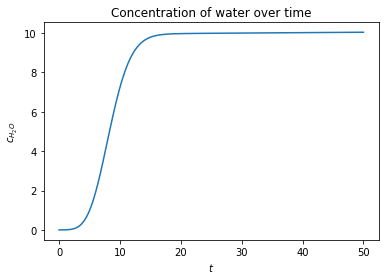
\includegraphics[width=.5\textwidth]{water.png}
	\caption{The result of Model 2}\label{fig:result}
\end{figure}%---------------------------------------------

再来一个伪代码,默认样式为\texttt{隐藏行号的三线表形式的伪代码}

可在\verb|ldmcm.sty|中修改样式,更详细的用法请参考algorithm2e宏包文档
%%%%%%%%%%伪代码%%%%%%%%%%%%%%%%%%%%%%

\begin{algorithm}[H]
	\KwIn{输入}
	\KwOut{输出 }
	initialization\;
	\While{not at end of this document}{
		read current\;
		\Repeat{this end condition}{
			do these things\;
		}
		\eIf{understand}{
			go to next section\;
			current section becomes this one\;
		}{
			go back to the beginning of current section\;
		}
		\Do{this end condition}{
			do these things\;
		}
	}
	\caption{How to write algorithms}
\end{algorithm}
%%%%%%%%%%伪代码%%%%%%%%%%%%%%%%%%%%%%


\clearpage
\subsection{Commetary on Model 2}
The instance of long and wide tables are shown in Table \ref{tb:longtable}.

% 长表格示例,更多用法请参考 longtable 宏包文档
% 以下环境及对应参数可实现表格内的自动换行与表格的自动断页
% 您也可以选择自行载入 tabularx 宏包,并通过 X 参数指定对应列自动换行
\begin{longtable}{ p{4em} p{14em} p{14em} }
	\caption{Basic Information about Three Main Continents (scratched from Wikipedia)}
	\label{tb:longtable}                                                                                                                      \\
	\toprule
	Continent                                                  & Description                                                    & Information \\
	\midrule
	Africa                                                     & Africa Continent is surrounded by the Mediterranean Sea to the
	north, the Isthmus of Suez and the Red Sea to the northeast, the Indian
	Ocean to the southeast and the Atlantic Ocean to the west. &
	At about 30.3 million km$^2$ including adjacent islands, it covers 6\%
	of Earth's total surface area and 20\% of its land area. With 1.3
	billion people as of 2018, it accounts for about 16\% of the world's
	human population.                                                                                                                         \\
	\midrule
	Asia                                                       & Asia is Earth's largest and most populous continent which
	located primarily in the Eastern and Northern Hemispheres.
	It shares the continental landmass of Eurasia with the continent
	of Europe and the continental landmass of Afro-Eurasia with both
	Europe and Africa.                                         &
	Asia covers an area of 44,579,000 square kilometres, about 30\%
	of Earth's total land area and 8.7\% of the Earth's total surface
	area. Its 4.5 billion people (as of June 2019) constitute roughly
	60\% of the world's population.                                                                                                           \\
	\midrule
	Europe                                                     & Europe is a continent located entirely in the Northern
	Hemisphere and mostly in the Eastern Hemisphere. It comprises the
	westernmost part of Eurasia and is bordered by the Arctic Ocean to
	the north, the Atlantic Ocean to the west, the Mediterranean Sea to
	the south, and Asia to the east.                           &
	Europe covers about 10,180,000 km$^2$, or 2\% of the Earth's surface
	(6.8\% of land area), making it the second-smallest
	continent. Europe had a total population of about 741 million (about
	11\% of the world population) as of 2018.                                                                                                 \\
	\bottomrule
\end{longtable}





\section{Model 3}
%===============================================第四部分=============================================
\section{Test the Model}
\subsection{Sensitivity  Analysis}
\subsection{Robustness Analysis}
\texttt{这部分很重要,不能缺!}








%==============================================第五部分================================================
\section{Conclusion}
\subsection{Summary of Results}

\subsection{Strengths}%------------------优点----------------
\begin{itemize}
	%1. 有灵敏度分析与稳健性分析
	\item The sensitivity analysis of the model demonstrates the effectiveness of the model under different parameter combinations and prove the robustness of the mod
	\item Second one ...
\end{itemize}

\subsection{Weaknesses and Improvements}%---------------缺点与改进---------------------
\begin{itemize}
	\item The analysis of fish migration can be more accurate if we have more complete data;
	\item Some approximate analysis methods are applied to model the management of fishing
	      companies, which may lead to a situation contrary to the actual one  in extreme cases.
	\item 此处引用了LLM.\upcite{openai2024chatgpt}
\end{itemize}




% 以下为信件/备忘录部分,不需要可自行去掉========================================================================
% 如有需要可将整个 letter 环境移动到文章开头或中间
% 请在第二个花括号内填写标题,如「信件」(Letter)或「备忘录」(Memorandum)
\begin{letter}{Memorandum}
	\begin{flushleft}  % 左对齐环境,无首行缩进
		\textbf{To:} Heishan Yan\\
		\textbf{From:} Team 1234567\\
		\textbf{Date:} October 1st, 2019\\
		\textbf{Subject:} A better choice than MS Word: \LaTeX
	\end{flushleft}

	In the memo, we want to introduce you to an alternate typesetting program to the prevailing MS Word: \textbf{\LaTeX}. In fact, the history of \LaTeX\ is even longer than that of MS Word. In the 1970s, the famous computer scientist Donald Knuth first came out with a typesetting program,  named \TeX\ \ldots

	Firstly, \ldots

	Secondly, \ldots

	Lastly, \ldots

	According to all those mentioned above, it is really worth to have a try on \LaTeX!
\end{letter}

%=================================================================================================================




% 参考文献,直接把bib格式粘贴到References.bib里面,此处无需改动!!!!!!!!!!!!!!!!!!
\bibliographystyle{unsrt} %规定了参考文献的格式
\begin{center}
	\bibliography{references.bib} %调出LaTeX生成参考文献列表
\end{center}
%=====================================================================================



% 以下为附录内容
% 如您的论文中不需要附录,请自行删除
\begin{subappendices}  % 附录环境

	\section{Appendix A: Further on \LaTeX}
	To clarify the importance of using \LaTeX\ in MCM or ICM, several points need to be covered, which are \ldots

	To be more specific, \ldots

	All in all, \ldots

	Anyway, nobody \textbf{really} needs such appendix \ldots

	\section{Appendix B: Program Codes}
	Here are the program codes we used in our research.

	% 代码环境示例三则
	% 如您的论文不需要展示代码,请删除
	% 更多用法,请参考 listings 宏包文档

	% Python 代码示例
	\lstinputlisting[language=python]{code/example.py}

	% MATLAB 代码示例
	\lstinputlisting[language=matlab]{code/example.m}

	\section{Appendix C: Report on Use of AI}
	% 人工智能的报告
	1. OpenAI ChatGPT (Nov 5, 2023 version, ChatGPT-4)

	Query1: <insert the exact wording you input into the AI tool>
	
	Output: <insert the complete output from the AI tool>

	2. OpenAI Ernie (Nov 5, 2023 version, Ernie 4.0)
	
	Query1: <insert the exact wording of any subsequent input into the AI tool>
	
	Output: <insert the complete output from the second query>
	
	3. Github CoPilot (Feb 3, 2024 version)
	
	Query1: <insert the exact wording you input into the AI tool>
	
	Output: <insert the complete output from the AI tool>
	
	4. Google Bard (Feb 2, 2024 version)
	
	Query: <insert the exact wording of your query>
	
	Output: <insert the complete output from the AI tool>
	

\end{subappendices}  % 附录内容结束

\end{document}  % 结束
